% G07 - ECOM060 - Fase 2, Entrega 03: instrumentacao em malha aberta (medicao ideal x real)
% Compilar com: xelatex relatorio.tex (duas vezes)
\documentclass[10pt,a4paper]{article}
\usepackage[margin=1.6cm,top=1.4cm,bottom=1.6cm]{geometry}
\usepackage{fontspec}
\setmainfont{TeX Gyre Termes}
\usepackage{amsmath,amssymb}
\usepackage{graphicx,booktabs,tabularx,multirow,array,xcolor}
\usepackage[font=small,labelfont=bf,labelsep=period]{caption}
\usepackage{enumitem}
\usepackage{newunicodechar}
\usepackage{placeins}

\newunicodechar{Ω}{\ensuremath{\Omega}}
\newunicodechar{→}{\ensuremath{\to}}
\newunicodechar{×}{\ensuremath{\times}}
\newunicodechar{·}{\ensuremath{\cdot}}
\newunicodechar{≤}{\ensuremath{\le}}
\newunicodechar{≈}{\ensuremath{\approx}}
\newunicodechar{°}{\ensuremath{^\circ}}
\newunicodechar{σ}{\ensuremath{\sigma}}
\newunicodechar{µ}{\ensuremath{\mu}}
\usepackage[hidelinks]{hyperref}
\renewcommand{\figurename}{Figura}
\renewcommand{\tablename}{Tabela}
\renewcommand{\refname}{Referências}
\setlist{nosep,leftmargin=*}
\setlength{\parskip}{2pt}
\newcolumntype{Y}{>{\raggedright\arraybackslash}X}
\makeatletter\let\inputtab\@@input\makeatother
\newcommand{\R}[1]{\FloatBarrier\par\medskip\noindent{\large\bfseries #1}\par\smallskip}
\emergencystretch=3em\sloppy
\begin{document}
\begin{center}
{\Large\bfseries Instrumentação em malha aberta: corrente de fase do motor BLDC MOONS' R42BLD30L3}\\[2pt]
Grupo G07 — Fase 2, Entrega 03 — ECOM060 Instrumentação Eletrônica (UFAL, 2026.2)\\[4pt]
\begin{tabular}{ll}\toprule Nome completo & Matrícula\\\midrule
Nícolas De Almeida Souza & 23111883\\ Lucas Momesso Alves & 22112804\\ Cláudio Henrique da Costa Santos & 20211850\\\bottomrule\end{tabular}
\end{center}

\R{Ponto de partida e escolha do sensor}
A planta é o equivalente elétrico validado na E02 \cite{e02} do modelo da E01 \cite{e01} (\texttt{modelo\_equivalente.tse}), executado no Virtual HIL (HIL101) e lido pelo HIL SCADA. A grandeza a medir (Anexo da orientação) é a \textbf{corrente de fase} $i_a$. Das duas tecnologias permitidas, escolhemos o \textbf{sensor de efeito Hall}: é a tratada no livro-texto (Aguirre, Seções 7.6 e 8.2.1, Fig.~8.17 \cite{aguirre}), já entrega uma tensão proporcional à corrente (sem amplificador diferencial externo, que o shunt exigiria) e é isolada do barramento de 36 V. O componente é o ACS712ELCTR-20A-T \cite{acs712}: CI Hall com condutor primário de 1,2 m$\Omega$, saída $V_Q + S\,i$ com $V_Q=2{,}5$ V e $S=100$ mV/A. A versão de $\pm$5 A saturaria na partida (6,4 A, R1).

\begin{figure}[!htbp]\centering
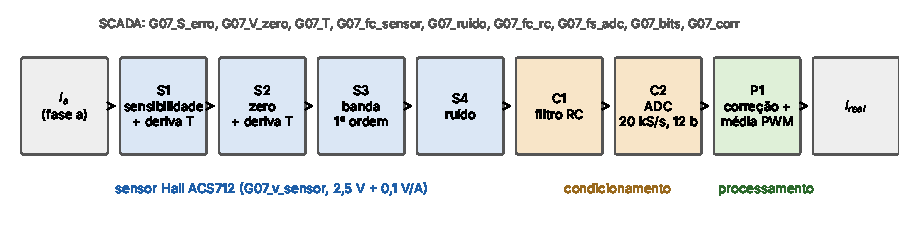
\includegraphics[width=\textwidth]{figuras/fig_cadeia.pdf}
\caption{Cadeia de medição no \texttt{modelo\_instrumentado.tse}. O primário do sensor (\texttt{G07\_iS}, \texttt{Current Measurement}) está em série com a fase $a$. Caminho ideal: \texttt{Gain} = 1 (\texttt{G07\_Med\_ideal}). Caminho real: um bloco por característica, cada um ajustado por um \texttt{SCADA Input}.}\label{fig:cadeia}
\end{figure}

\R{R1. Demanda de instrumentação}
Os valores vêm do modelo da E01, executado pelo seu equivalente da E02 no VHIL, que o reproduz dentro dos critérios da E02: pico de corrente na partida de 6,4 A (6,3 A no trifásico da E01), $\tau_e$ = 1,19 ms e 3658 rpm no degrau (Fig.~\ref{fig:dem}).

\begin{figure}[!htbp]\centering
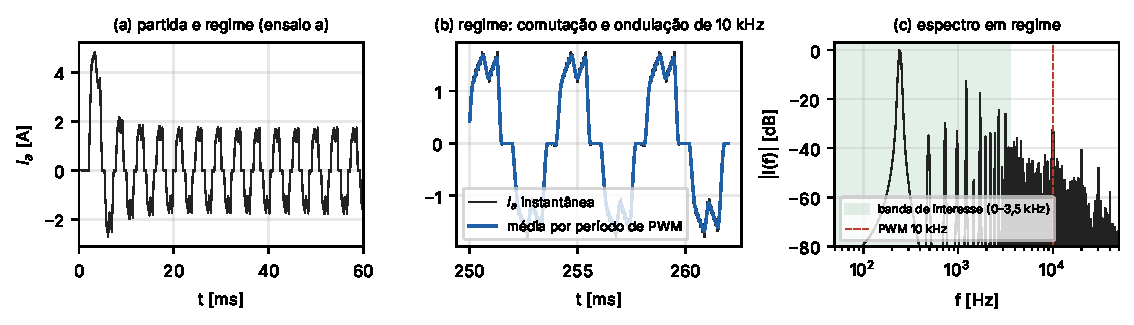
\includegraphics[width=\textwidth]{figuras/fig_demanda.pdf}
\caption{Corrente de fase no ensaio (a) (VHIL). (b) Em regime, a corrente tem a forma de 120° com comutações a cada 60° elétricos e ondulação de PWM de 0,68 A p-p a 10 kHz. (c) 99,8 \% da potência (sem a média) está abaixo de 3,5 kHz; a raia de 10 kHz é a ondulação do PWM.}\label{fig:dem}
\end{figure}

\begin{table}[!htbp]\centering\footnotesize
\caption{Requisitos da medição, obtidos do modelo.}\label{tab:dem}
\begin{tabularx}{\textwidth}{p{2.6cm}p{3.3cm}Y}\toprule
Grandeza & Requisito & Origem no modelo\\\midrule
Faixa & $\pm$10 A (com margem) & E01: corrente de pico de catálogo 5 A ($T_{max}/k$), contínua 1,67 A e $i_0$ = 1,675 A a 4000 rpm (R2 da E01); a partida do modelo passa do catálogo: 5,83 A no médio e 6,3 A no trifásico da E01, 6,4 A no equivalente (três fases), 4,8 A na fase $a$\\
Banda de interesse & 0 a 3,5 kHz & $f_e = 244$ Hz a 3658 rpm ($p=4$); 5.ª, 7.ª, 11.ª e 13.ª harmônicas até 3,2 kHz; 99,8 \% da potência $\le$ 3,5 kHz. A ondulação de 10 kHz \emph{não} é de interesse: o valor útil é a média por período de PWM, que é a que gera torque\\
Resolução & $\le$ 40 mA & pulso de carga de 0,02 N·m (terceiro ensaio da E01): $\Delta i$ = 0,274 A no médio da E01 e $\Delta i_{rms}$ = 0,21 A na fase $a$ (ensaio c); resolver 1/5 dessa variação\\
Incerteza & viés $\le$ 25 mA; aleatória $\le$ 70 mA rms & viés $\le$ 2 \% de 1,14 A (valor eficaz em regime; erro de torque de 2 \% via $T_e = k\,i$); aleatória $\le$ 1/3 de $\Delta i_{rms}$ por amostra\\
Atraso & $\le$ 100 µs & um período de PWM; E01: $\tau_e = L_{LL}/R_{LL}$ = 1,188 ms e setor de comutação de 0,625 ms a 4000 rpm\\\bottomrule
\end{tabularx}
\end{table}

\R{R2. Sensor ideal e sensor real}
\textbf{Estrutura funcional (Cap.~2).} Elemento primário: o condutor de 1,2 m$\Omega$ gera o campo $B = k_B\,i$. Transdução: tensão de Hall $V_H = K_H\,I_c\,B$ (Eq.~7.59, com corrente de excitação $I_c$ constante interna), amplificada e deslocada para $V_Q$. Entradas espúrias (Seção 2.4): a temperatura é \emph{modificante} (altera $K_H$, logo a sensibilidade) e \emph{interferente} (desloca o zero); campos externos e a deformação (efeito piezorresistivo, Eq.~7.60) são interferentes. Modelo do sensor real:
\begin{equation}
v_s = \Big[V_Q + e_Q + \tfrac{\partial V_Q}{\partial T}(T-25)\Big] + \Big[S(1+e_S) + \tfrac{\partial S}{\partial T}(T-25)\Big]\, i \;\xrightarrow{\;\frac{1}{1+s/\omega_s}\;}\; +\;\sigma_v\,n(t).
\end{equation}

\begin{table}[!htbp]\centering\footnotesize
\caption{Características do sensor e do condicionamento: valor ideal, valor real adotado e fonte. Cada uma está em um bloco do caminho real e é ajustada pelo SCADA Input indicado (valor 0 = característica desligada; $T$ = 25 °C anula as derivas).}\label{tab:car}
\begin{tabularx}{\textwidth}{p{3.0cm}p{1.9cm}p{2.8cm}p{2.3cm}Y}\toprule
Característica (livro) & Ideal & Real (padrão) & SCADA / bloco & Fonte e justificativa\\\midrule
Sensibilidade (3.3.1) e desvio de sensibilidade (3.3.8) & 100 mV/A & 101,5 mV/A ($e_S$ = +1,5 \%); $-$0,004 mV/A/°C & \texttt{G07\_S\_erro}, \texttt{G07\_T} / S1 & erro total $E_{TOT}$ = $\pm$1,5 \% e inclinação da sensibilidade de 25 a 150 °C \cite{acs712}; $T$ = 60 °C (placa do inversor), estimativa nossa dentro da faixa da E01 (ambiente de 0 a 50 °C, motor até 120 °C)\\
Desvio de zero (3.3.8) & 2,500 V & +10 mV; $-$0,07 mV/°C & \texttt{G07\_V\_zero}, \texttt{G07\_T} / S2 & inclinação do zero \cite{acs712}; 10 mV (0,1 A) é estimativa nossa de desvio inicial, coerente com o erro total\\
Resposta dinâmica (4.2.2) & instantânea & 1.ª ordem, 80 kHz & \texttt{G07\_fc\_sensor} / S3 & banda de $-$3 dB e tempo de subida de 3,5 µs \cite{acs712}; o livro indica 25 kHz típicos para Hall \cite{aguirre}\\
Ruído (5.4) & nulo & 10 mV rms branco a 200 kS/s & \texttt{G07\_ruido} / S4 & 11 mV p-p em 2 kHz de banda \cite{acs712} ⇒ 1,8 mV rms; espalhado até 100 kHz: $1{,}8\sqrt{100/(2\cdot\pi/2)}\approx$ 10 mV\\
Faixa (3.3.6) & ilimitada & 0 a 5 V ($\pm$25 A) & fixa, no ADC (C2) & saída limitada à alimentação de 5 V; não é ajustável nem é exercitada, porque o pico de 6,4 A fica longe de 25 A\\
Filtro anti-aliasing (6.2.1) & — & RC de 1.ª ordem, 15 kHz & \texttt{G07\_fc\_rc} / C1 & projeto (R3)\\
Conversão A/D: amostragem e resolução (3.3.2) & contínua & 20 kS/s síncrona; 12 bits, 5 V & \texttt{G07\_fs\_adc}, \texttt{G07\_bits} / C2 & projeto (R3); LSB = 1,22 mV = 12,2 mA\\
Processamento (2.5.3, 6.2.2) & — & correção calculada + média por período & \texttt{G07\_corr} / P1 & projeto (R3)\\\bottomrule
\end{tabularx}
\end{table}

Não foram incluídas: não linearidade e histerese, desprezíveis no datasheet frente às demais (o ACS712 tem histerese magnética quase nula \cite{acs712}), e o acoplamento de campos externos, que depende da montagem e não tem valor publicado (fica como entrada interferente citada, sem bloco).

\textbf{Implementação no TyphoonSim (inventário).} Primário do sensor: \texttt{core/Current Measurement} (\texttt{G07\_iS}, 5 µs) em série com a fase $a$; grandeza real: \texttt{core/Probe} \texttt{G07\_i\_verdadeira}; caminho ideal: \texttt{core/Gain} = 1 e \texttt{core/Probe} \texttt{G07\_i\_ideal}; ajustes: nove \texttt{core/SCADA Input}; ligações por \texttt{tag} Goto/From; leituras: \texttt{core/Probe}. Os blocos S1 a P1 são \texttt{core/C function} (5 µs, de 3 a 58 linhas cada; Apêndice A): os blocos nativos de ganho, filtro e quantização têm parâmetros fixos na compilação, e a orientação pede ajuste pelo SCADA com o modelo rodando. Cada bloco também calcula sua saída \texttt{iso}: a corrente medida com \emph{só} aquela característica, convertida para ampères (probes \texttt{G07\_iso\_*}). Assim, uma captura mostra a contribuição isolada de cada uma (R4), e os blocos S3, S4 e C2 calculam também os três níveis exagerados do R5 (probes \texttt{G07\_R5\_*}).

\R{R3. Circuitos auxiliares e processamento}
\begin{table}[!htbp]\centering\footnotesize
\caption{Condicionamento e processamento: o que atende e a que método do Cap.~2 corresponde.}\label{tab:cond}
\begin{tabularx}{\textwidth}{p{3.3cm}Yp{3.6cm}}\toprule
Circuito / processamento & Projeto e requisito atendido & Método (Cap.~2)\\\midrule
Excitação e saída raciométrica, ADC com $V_{ref}$ = $V_{CC}$ & o elemento Hall é excitado por corrente constante interna ao CI (Seção 8.2.1), alimentado por $V_{CC}$ = 5 V; $V_Q$ e $S$ são proporcionais a $V_{CC}$ \cite{acs712}, e usando a mesma alimentação como referência do ADC a variação de $V_{CC}$ se cancela na conversão. No modelo, $V_{CC}$ é ideal, então este item é de projeto e não foi simulado & insensibilidade inerente (2.5.1) / entradas em oposição (2.5.4)\\
Filtro RC anti-aliasing, 15 kHz & atenua o ruído de banda larga e a ondulação acima de $f_s/2$ = 10 kHz; em 3,5 kHz perde só 2,6 \% (ganho 0,974) e atrasa 10 µs: banda do R1 & filtragem (2.5.2; 6.2.1)\\
ADC 12 bits, 20 kS/s síncrono com a portadora & duas amostras por período de PWM, no vale e no pico da portadora, onde a corrente passa pelo valor médio do período; LSB de 12 mA $<$ 40 mA (resolução do R1) & filtragem (amostragem síncrona)\\
Conversão V → A com correção calculada & $\hat\imath = (v - \hat V_Q)/\hat S$, com $\hat V_Q = V_Q + e_Q + \partial_T V_Q\,(T-25)$ e $\hat S = S(1+e_S)+\partial_T S\,(T-25)$: $e_Q$ e $e_S$ da calibração estática (3.2) e $T$ medida na placa; remove o viés de 75 mA (R1: $\le$ 25 mA) & correções calculadas (2.5.3)\\
Média móvel de 2 amostras (1 período de PWM) & média do vale e do pico: o valor útil (média por período); reduz o ruído de $1/\sqrt2$; atraso de meia amostragem + meio período ≈ 50 µs ($\le$ 100 µs) & filtragem discreta (2.5.2; 6.2.2)\\
Sensor em malha aberta (não compensado) & a realimentação negativa de fluxo (sensor Hall em malha fechada) reduziria derivas e não linearidade, mas não é necessária com a correção acima & realimentação (2.5.5), não usada\\\bottomrule
\end{tabularx}
\end{table}

\R{R4. Ensaio em malha aberta}
Os três ensaios da E01 foram aplicados à planta no VHIL e gravados pelo Capture do HIL SCADA (0,3 s, 100 kS/s; gatilho na partida): (a) degrau de $d$ do repouso; (b) condição inicial não nula ($d=0$ a partir de 150 ms, com a corrente indo a zero); (c) pulso de carga de 0,02 N·m entre 100 e 200 ms. A medição é feita em malha aberta: o sinal medido não realimenta o controle.

\begin{figure}[!htbp]\centering
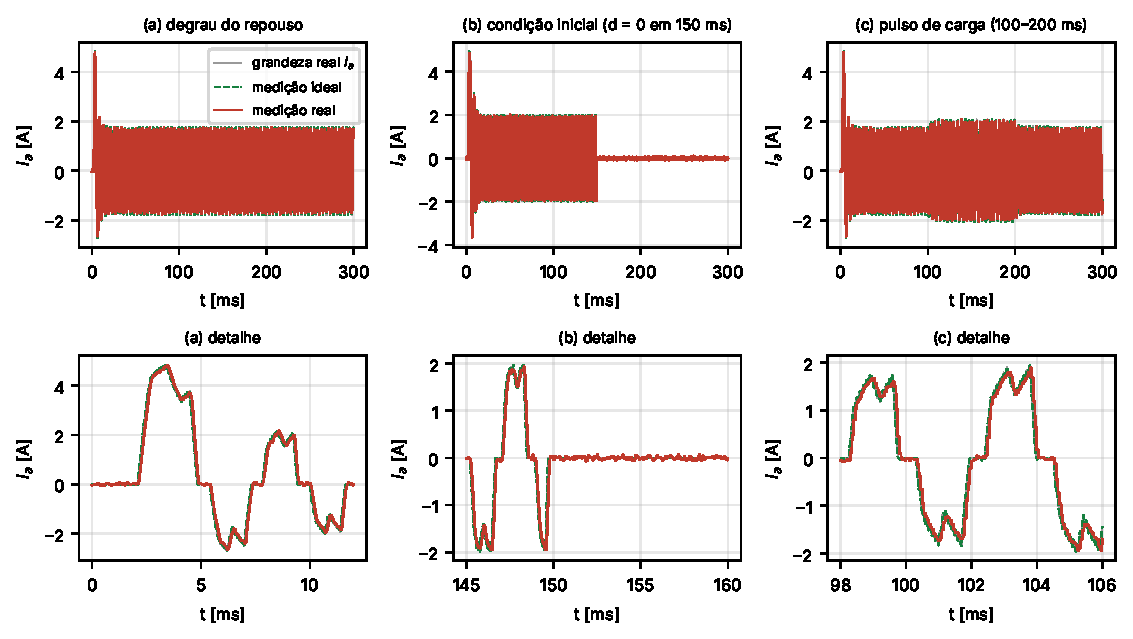
\includegraphics[width=\textwidth]{figuras/fig_ensaios.pdf}
\caption{Grandeza real (cinza), medição ideal (verde tracejado, sobreposta à real) e medição real (vermelho) nos três ensaios; embaixo, detalhes. A medição real acompanha a média por período de PWM, com atraso de 60 µs e degraus de 50 µs (amostragem a 20 kS/s).}\label{fig:ens}
\end{figure}

\begin{table}[!htbp]\centering\footnotesize
\caption{Ideal × real nos três ensaios (janelas: (a) 200–300 ms, (b) 200–300 ms com corrente nula, (c) 120–200 ms, durante o pulso). A medição ideal coincide com a grandeza real em todas as amostras (erro máximo 0 A). Referência da real: média da grandeza real por período de PWM, o valor de interesse do R1. Erro relativo = erro rms / valor eficaz da referência.}\label{tab:r4}
\begin{tabular}{lrrrr}\toprule
Grandeza & Ideal (a, b, c) & Real (a) & Real (b) & Real (c)\\\midrule
\inputtab tabelas/tab_r4.tex \bottomrule
\end{tabular}
\end{table}

\begin{figure}[!htbp]\centering
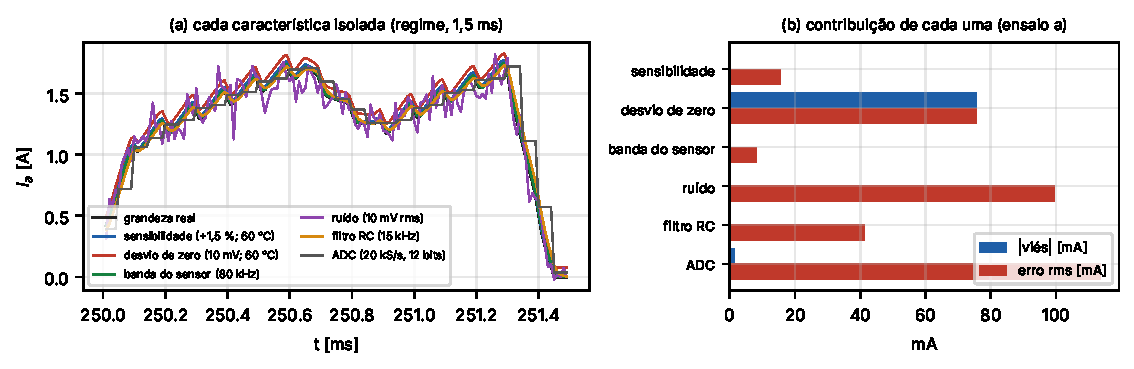
\includegraphics[width=\textwidth]{figuras/fig_contribuicoes.pdf}
\caption{Cada característica ligada isoladamente (saídas \texttt{iso} dos blocos; ensaio a, regime). Erro em relação à corrente instantânea.}\label{fig:contr}
\end{figure}

\begin{table}[!htbp]\centering\footnotesize
\caption{Contribuição de cada característica isolada (ensaio a, 200–300 ms): viés, erro rms em relação à corrente instantânea e erro rms das médias por período de PWM.}\label{tab:contr}
\begin{tabular}{lrrrl}\toprule
Característica (só ela ligada) & Viés [mA] & Erro rms [mA] & Erro rms na média [mA] & Explicação\\\midrule
\inputtab tabelas/tab_contr.tex \bottomrule
\end{tabular}
\end{table}

\textbf{Leitura.} A medição ideal coincide com a grandeza real em todas as amostras (erro máximo 0). Na real, o viés fica em 0,5 a 2 mA nos três ensaios porque a correção calculada remove o desvio de zero e o erro de sensibilidade. Com a corrente nula, no fim do ensaio (b), ela marca 1,2 mA; sem a correção marcaria 75,5 mA. O erro rms contra a média por período é de 58 mA, depois de descontado o atraso de 60 µs. Ele vem do ruído filtrado pelo RC e pela média ($10\,\text{mV}\sqrt{\pi/2\cdot15/100}/\sqrt2 \approx 3{,}4$ mV, ou seja 34 mA), da quantização (3,5 mA) e da forma de onda nas comutações. A medição atende ao viés, à resolução e ao atraso do R1. O erro aleatório de 58 mA fica abaixo dos 70 mA pedidos. No ensaio (c), a variação de corrente eficaz causada pelo pulso é medida como 0,208 A, contra 0,209 A da grandeza real.

\R{R5. Exacerbação e síntese}
Foram exagerados três níveis de três características, cada uma isolada, em regime. As previsões foram calculadas \emph{antes} da simulação com as expressões abaixo, sobre o espectro da corrente medido no R1:
\begin{itemize}
\item \textbf{banda:} $e_{rms}^2 = \sum_f |1 - H(f)|^2 |I(f)|^2$, com $H = 1/(1+jf/f_c)$ (Eq.~de 1.ª ordem, Seção 4.4.2);
\item \textbf{ruído:} $e_{rms} = \sigma_v/S$;
\item \textbf{quantização:} $e_{rms} = q/\sqrt{12}$, com $q = 5\,\text{V}/(2^N S)$ (ruído de quantização uniforme).
\end{itemize}

\begin{figure}[!htbp]\centering
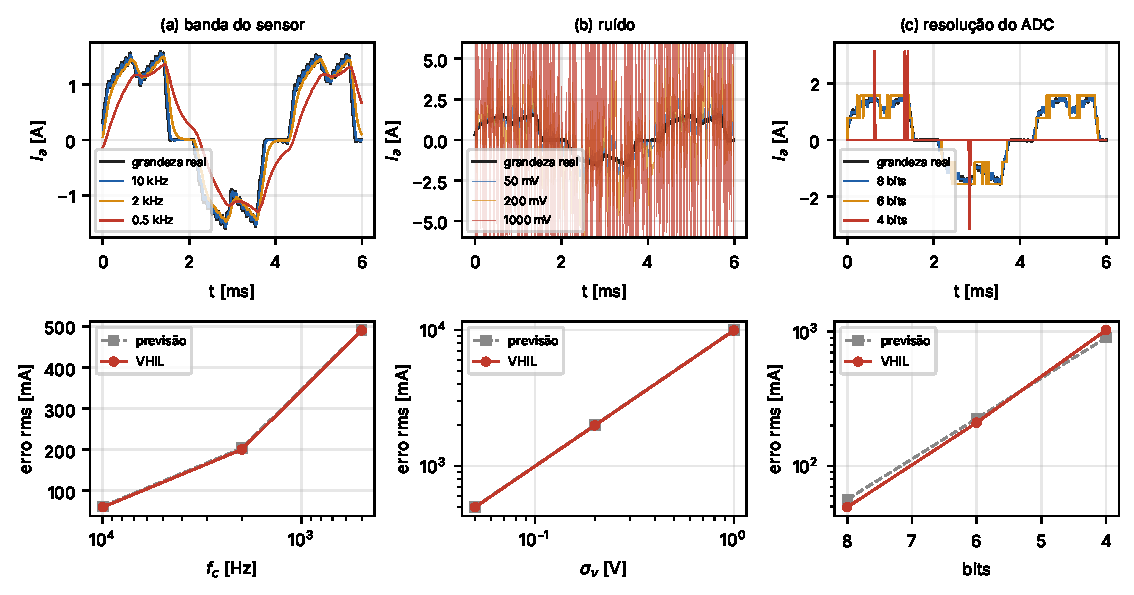
\includegraphics[width=\textwidth]{figuras/fig_exacerbacao.pdf}
\caption{R5 no VHIL (captura de 50 ms em regime). Em cima, a corrente medida em cada nível; embaixo, o erro rms previsto e o simulado.}\label{fig:r5}
\end{figure}

\begin{table}[!htbp]\centering\footnotesize
\caption{Previsão × resultado do R5 (erro rms em relação à grandeza real, cujo valor eficaz é 1,03 A nesta captura).}\label{tab:r5}
\begin{tabularx}{\textwidth}{p{2.4cm}rrrY}\toprule
Característica e nível & Previsto [mA] & VHIL [mA] & Atraso & Explicação física e algébrica\\\midrule
\inputtab tabelas/tab_r5.tex \bottomrule
\end{tabularx}
\end{table}

\textbf{Síntese.} Na configuração real, o que mais compromete a informação é o \textbf{desvio de zero}. Sozinho, ele dá 75 mA de viés (6,6 \% do valor eficaz em regime) e não diminui com média nem com filtro, porque é sistemático. Ele importa para todo uso que depende do \emph{valor médio}: estimativa do torque ($T_e = k\,i$), da potência e malha de corrente. Por isso a correção calculada é indispensável, e ela o reduz a 1 mA. Entre as características exageradas, o \textbf{ruído} é o mais nocivo. Com 1 V rms o erro chega a 10 A, quase 10 vezes a própria corrente: ele importa para a proteção de sobrecorrente (disparos falsos) e para qualquer leitura amostra a amostra. A banda baixa ($f_c$ = 0,5 kHz) quase não muda o valor médio, mas atrasa 230 µs e apaga a forma da comutação, o que importa para a malha de corrente e para detectar picos. A resolução de 4 bits zera a leitura em regime, porque ±1,8 A fica dentro de um degrau de 3,1 A: o instrumento continua respondendo a picos grandes, mas perde a informação de regime.

\R{R6. Repetibilidade (roteiro)}
\begin{enumerate}
\item Instalar o Typhoon HIL Control Center \textbf{2026.3}. Arquivos (pasta \texttt{entregas/fase-2/e3-instrumentacao/simulacao/}): \texttt{modelo\_instrumentado.tse} (modelo) e \texttt{painel\_instrumentado.cus} (painel do HIL SCADA).
\item Abrir o \texttt{.tse} no Schematic Editor, perspectiva \textbf{tempo real}. Em \emph{Model > Model settings > Model initialization}, colar o bloco do ensaio (Tab.~\ref{tab:rot}), compilar e conferir no console \texttt{G07 E03: sensor Hall S0=0.100 V/A} e \texttt{modo de ensaio = …}.
\item Abrir o HIL SCADA, carregar \texttt{modelo\_instrumentado Target files/modelo\_instrumentado.cpd} em \textbf{Virtual HIL} e abrir \texttt{painel\_instrumentado.cus}. As caixas trazem os valores reais da Tab.~\ref{tab:car}. Após cada nova compilação, usar \emph{Model > Reload Model}.
\item R4: no Capture/Scope, preset \textbf{Default} (0,3 s, 100 kS/s, 13 sinais, gatilho em \texttt{n}, borda de subida, 20, \emph{Use first trigger}). Com a simulação parada, clicar no botão de captura com gatilho (\textbf{T↑}) e depois em \emph{Start simulation}. Exportar em CSV (primeiro ícone vermelho da barra inferior, \emph{Save data}).
\item R5: com o bloco do ensaio (a) e a simulação rodando há uns 2 s, escolher o preset \textbf{R5} (0,05 s, 11 sinais) e clicar em \textbf{T↑} (ou em \textbf{F} para forçar o gatilho). Exportar em CSV.
\item Demonstração ao vivo: com o modelo rodando, mudar as caixas do painel (por exemplo \texttt{G07\_corr} = 0, \texttt{G07\_ruido} = 200, \texttt{G07\_fc\_sensor} = 0,5, \texttt{G07\_bits} = 4) e observar \texttt{G07\_i\_real} contra \texttt{G07\_i\_verdadeira}.
\end{enumerate}
\begin{table}[!htbp]\centering\footnotesize
\caption{Bloco do \emph{Model initialization} (de \texttt{g07\_modo} a \texttt{g07\_d0}) e resultado esperado. Linhas comuns a todos: \texttt{g07\_d\_ini = 0.0}, \texttt{g07\_d\_deg = 0.7074}, \texttt{g07\_t\_deg = 0.0}, \texttt{g07\_t\_ci = 0.15}, \texttt{g07\_d\_ci = 0.0}, \texttt{g07\_Td = 0.02}, \texttt{g07\_t\_p1 = 0.10}, \texttt{g07\_t\_p2 = 0.20}, \texttt{g07\_d0 = 0.7074}.}\label{tab:rot}
\begin{tabularx}{\textwidth}{p{3.4cm}p{2.0cm}p{1.9cm}Y}\toprule
Ensaio & Muda & CSV & Resultado esperado\\\midrule
(a) degrau do repouso & \texttt{g07\_modo = 1} & \texttt{e3\_a.csv} & $n$ ≈ 3658 rpm; $i_a$ eficaz 1,14 A; real: viés ≈ 0,5 mA, erro rms ≈ 58 mA (com atraso de 60 µs descontado)\\
(b) condição inicial & \texttt{g07\_modo = 2} & \texttt{e3\_b.csv} & corrente nula após 150 ms; real marca ≈ 1 mA (sem correção, 75 mA)\\
(c) pulso de carga & \texttt{g07\_modo = 3} & \texttt{e3\_c.csv} & $\Delta i_{rms}$ ≈ 0,21 A no pulso, real e ideal\\
R5 & \texttt{g07\_modo = 1} & \texttt{e3\_r5.csv} & erros da Tab.~\ref{tab:r5}\\\bottomrule
\end{tabularx}
\end{table}

\begin{thebibliography}{9}\small
\bibitem{aguirre} L. A. Aguirre. \emph{Fundamentos de Instrumentação}. São Paulo: Pearson, 2013 (Caps. 2 a 7; Seções 7.6 e 8.2.1).
\bibitem{acs712} Allegro MicroSystems. \emph{ACS712: Fully Integrated, Hall Effect-Based Linear Current Sensor IC with 2.1 kVRMS Isolation and a Low-Resistance Current Conductor}, datasheet ACS712-DS. Disponível em: \url{https://www.allegromicro.com/-/media/files/datasheets/acs712-datasheet.ashx}.
\bibitem{e01} G07. Caracterização da planta no domínio de origem: motor BLDC MOONS' R42BLD30L3 (Fase 2, Entrega 01). ECOM060, UFAL, 2026.
\bibitem{e02} G07. Equivalente elétrico no TyphoonSim: motor BLDC MOONS' R42BLD30L3 (Fase 2, Entrega 02). ECOM060, UFAL, 2026.
\bibitem{ty} Typhoon HIL. Schematic Editor, HIL SCADA e Capture/Scope — documentação da versão 2026.3.
\end{thebibliography}

\appendix
\section*{Apêndice A. Código externo: blocos \texttt{C function}}
O código completo está no próprio \texttt{.tse} e, para leitura, em \texttt{simulacao/codigo\_c\_functions.md}. Todos os blocos executam a 5 µs e leem do \emph{Model initialization} os parâmetros nominais (\texttt{g07\_S0} = 0,1 V/A, \texttt{g07\_VQ} = 2,5 V, derivas, \texttt{g07\_Tsen} = 5 µs e os níveis do R5). Cada um tem a saída principal, que segue a cadeia real, e a saída \texttt{iso}, que aplica só a sua característica à corrente verdadeira.
\begin{table}[!htbp]\centering\footnotesize
\begin{tabularx}{\textwidth}{p{2.9cm}p{2.6cm}Yp{0.8cm}}\toprule
Bloco & Entradas & Operação & Linhas\\\midrule
\texttt{G07\_S1\_sensibilidade} & $i$, $e_S$, $T$ & $v = S\,[1+e_S+\partial_TS\,(T-25)/S]\,i$ & 3\\
\texttt{G07\_S2\_zero} & $v$, $i$, $e_Q$, $T$ & $v \mathrel{+}= V_Q + e_Q + \partial_TV_Q\,(T-25)$ & 3\\
\texttt{G07\_S3\_banda} & $v$, $i$, $f_c$ & 1.ª ordem por Euler regressivo, $y_k = y_{k-1} + \frac{\omega T}{1+\omega T}(x_k-y_{k-1})$; mais 3 níveis do R5 & 23\\
\texttt{G07\_S4\_ruido} & $v$, $i$, $\sigma_v$ & $v \mathrel{+}= \sigma_v\,n_k$; $n_k$ gaussiano (soma de 6 uniformes do gerador de Park–Miller, método de Schrage, sem estouro de 32 bits); mais 3 níveis do R5 & 23\\
\texttt{G07\_C1\_filtro\_RC} & $v$, $i$, $f_c$ & 1.ª ordem, igual ao S3 & 11\\
\texttt{G07\_C2\_ADC} & $v$, $i$, $f_s$, $N$ & amostra a cada $1/(f_s T)$ passos (síncrono com a portadora), limita a 0–5 V e quantiza com $q = 5/2^N$; saída \texttt{novo} marca a amostra; mais 3 níveis do R5 & 58\\
\texttt{G07\_P1\_processamento} & $v$, \texttt{novo}, $e_S$, $e_Q$, $T$, \texttt{corr}, $f_s$ & $\hat\imath = (v-\hat V_Q)/\hat S$ com a correção calculada; média das últimas $f_s/f_{PWM}$ amostras & 27\\\bottomrule
\end{tabularx}
\end{table}
\end{document}
